\chapter{绪论}
\label{cha:intro}

\section{研究背景和意义}

自然语言处理(Natural Language Processing, NLP)是目前人工智能方兴未艾的领域之一.
一个完整的自然语言处理句子分析流程主要分为三个部分:1)词法分析;2)句法分析;3)语义分析.
其中词法分析包含了词性标注(Part-of-Speech Tagging)、命名实体识别(Named Entity Recognition, NER)以及消歧(Disambiguation)等子任务,中文中由于词语之间没有天然边界,还需要额外进行中文分词.
句法分析的目的是以句法树的形式刻画句子结构,主要包含了依存句法(Dependency Parsing)和成分句法(Constituency Parsing)分析这两种范式.
语义分析则是为了理解句子的内含语义,包含语义角色标注(Semantic Role Labeling, SRL)、语义依存分析(Semantic Dependency Parsing, SDP)和抽象语义表示(Abstract Meaning Representation, AMR)等子任务.

上述的三个流程通常以管道的方式进行,而句法分析作为连接词法和语义分析的中间步骤,具备十分重要的研究价值.
目前存在着多种句法分析文法,例如组合范畴文法(Combinatorial Categorical Grammars, CCGs),成分文法(Constituency Grammars or Context Free Grammars, CFGs),以及依存文法(Dependency Grammars).
其中依存文法对应的依存句法分析,和成分文法对应的成分句法分析是目前最常见的句法分析范式,也是本文主要的研究对象.

\begin{figure}[tb]
  \begin{center}
    \begin{dependency}%[arc edge, arc angle=80, text only label, label style={above}] %, hide label]
      %\begin{dependency} %[arc edge, arc angle=80] %, text only label, label style={above}] %, hide label]
      \begin{deptext}[column sep=.2cm] %[row sep=0.4cm, column sep=.22cm] %column sep=.2cm,
        \$$_0$ \& I$_1$ \& saw$_2$ \& Sarah$_3$ \& with$_4$ \&a$_5$ \& telescope$_6$ \\
        %\textsl{Gap:} \& $0.9$ \& $0.5$ \& $0.7$ \&[.4cm] $0.1$ \& $0.9$ \& $0.8$ \\
      \end{deptext}
      \depedge[edge style={black}]{3}{2}{nsubj}
      \depedge[edge style={black}]{3}{4}{dobj}
      \depedge[edge style={black}]{5}{7}{pobj}
      \depedge[edge style={black}]{7}{6}{det}
      \depedge[edge style={draw={rgb,255:red,76; green,114; blue,176}, thick}, label style={draw={rgb,255:red,76; green,114; blue,176}, text={rgb,255:red,76; green,114; blue,176}, semithick}]{1}{3}{root}
      \depedge[edge style={draw={rgb,255:red,76; green,114; blue,176}, thick}, label style={draw={rgb,255:red,76; green,114; blue,176}, text={rgb,255:red,76; green,114; blue,176}, semithick}]{3}{5}{prep}
    \end{dependency}
    \caption{
      一个完整依存树的例子.
      对于局部标注的场景,仅有一部分的弧被标注,例如图中两个粗蓝弧.
    }
    \label{fig:dep-tree-example} %
  \end{center}
\end{figure} %
依存句法分析的目的是识别句子中词语的修饰关系.
如图\ref{fig:dep-tree-example}所示,给定一个句子$\boldsymbol{x}=w_0,w_1,\cdots,w_n$,一棵依存树被定义为$\boldsymbol{t}=\{(i\rightarrow j,l)\mid 0\le i \le n,0 < j \le n,l \in \mathcal{L}\}$,其中$(i\rightarrow j,l)$是一条从头(head)$w_i$到修饰词(modifier)$w_j$的弧,弧的标签为$l \in \mathcal{L}$.
有标签树$\boldsymbol{t}$可以进一步被分解为$(\boldsymbol{y},\boldsymbol{l})$,即一棵无标签树$\boldsymbol{y}$和树上所有标签组成的序列$\boldsymbol{l}$.
得益于基准数据集宾州书库(Penn Treebank, PTB)的发布,以及深度学习技术的发展,目前依存句法分析技术得到了广泛研究.
其中计算自然语言学习会议(Conference on Computational Natural Language Learning, CoNLL)连续多年针对依存句法任务发布了评测任务,尤其是近年来依托通用依存(Universal Dependencies, UD) \citep{nivre-etal-2017-universal}项目发布的多语言评测比赛,大大推动了依存句法分析技术的进步.
由于结构简单、形式直观的特点,依存句法分析一直被广泛的应用在多个其他任务中,例如机器翻译 \citep{zhang-etal-2019-syntax}、关系抽取 \citep{song-etal-2019-leveraging}、意见挖掘 \citep{zhang-etal-2020-syntax}等等.

\begin{figure}[tb!]
	\centering
	\begin{subfigure}[b]{0.45\textwidth}
		\centering
		\begin{tikzpicture} [
				level distance=24pt,
				every tree node/.style={align=center,anchor=base},
				frontier/.style={distance from root=92pt},
				edge from parent/.style={draw,edge from parent path={(\tikzparentnode.south) {[rounded corners=0.5pt]-- ($(\tikzchildnode |- \tikzparentnode.south) + (0, -5pt)$) -- (\tikzchildnode)}}}
			]
			\Tree
			[.S
				[.NP I$_1$ ]
				[.ADVP really$_2$ ]
				[.VP love$_3$ [.NP this$_4$ game$_5$ ] ]
			];
		\end{tikzpicture}
		\caption{原始句法树}
		\label{fig:con-original-tree}
	\end{subfigure}
	\hfill
	\begin{subfigure}[b]{0.45\textwidth}
		\centering
		\begin{tikzpicture} [
				level distance=24pt,
				every tree node/.style={align=center,anchor=base},
				frontier/.style={distance from root=92pt},
				edge from parent/.style={draw,edge from parent path={(\tikzparentnode.south) {[rounded corners=0.5pt]-- ($(\tikzchildnode |- \tikzparentnode.south) + (0, -5pt)$) -- (\tikzchildnode)}}}
			]
			\Tree
			[.S
				[.$\textrm{S}^\ast$ [.NP I$_1$ ] [.ADVP really$_2$ ] ]
				[.VP
					[.$\textrm{VP}^\ast$ love$_3$ ]
					[.NP [.$\textrm{NP}^\ast$ this$_4$ ] [.$\textrm{NP}^\ast$ game$_5$ ] ]
				]
			];
		\end{tikzpicture}
		\caption{遵循乔姆斯基范式的左二叉化句法树}
		\label{fig:con-binaried-tree}
	\end{subfigure}
	\caption{
		成分句法树的例子.
		其中词性在这里被忽略
	}
	\label{fig:con-tree-full-figure}
\end{figure}

成分句法则旨在构建一个层次化的树结构.
如图\ref{fig:con-tree-full-figure},其中每个叶子结点是输入句子的每个词,而非终端结点作为区块(Constituents),如$\texttt{VP}_{3,5}$.
正式地,给定一个由$n$个词组成的句子$\boldsymbol{x}=w_1,\dots,w_{n}$,如图~\ref{fig:con-tree-original}所示,一棵成分句法树可以表示为$\boldsymbol{t}=\{((i, j),l)\mid 1\le i \le n,i \le j \le n,l \in \mathcal{L}\}$,其中$((i,j),l) \in \boldsymbol{t}$是一个包含$w_{i}...w_{j}$的区块,对应的句法标签为$l \in \mathcal{L}$.
本文中,为了方便模型处理,我们还将原始的树转换为了二叉树形式,如图~\ref{fig:con-binaried-tree}所示.
成分句法分析相比于依存句法而言,研究历史更加悠久,尽管目前没有依存句法技术那么流行,但是以其分析技术为基础衍生出了一系列在其他任务上的解析方法,例如UCCA语义分析 \citep{jiang-etal-2019-hlt}、嵌套命名实体识别 \citep{fu-etal-2021-nested}等等.

不同于传统句法分析方法十分依赖于离散特征的人工设计,由于深度神经网络的强大上下文编码能力,句法分析器的方法愈来愈有简单化的趋势.
其中依存句法分析器Biaffine Parser \citep{dozat-etal-2017-biaffine}正是符合这样的潮流:利用诸如双向LSTM或Transformer \citep{vaswani-2017-attention}等强大编码器得到上下文表示,然后采取一个简单的头选择训练损失函数训练每个词找到正确的头.
类似的,\citet{gaddy-etal-2018-whats}采用的成分句法分析器采用了一个二分类训练目标,判断每个位置是否能够组成一个区块.
由于其准确率高,速度快的特点,基于局部训练目标的分析器是目前最为流行的句法分析器.

然而,已有的句法分析器Biaffine Parser也存在一些固有的缺陷.
由于训练时没有显式的树结构约束,在解码时分析器仍然需要通过解码算法(例如Eisner算法、MST算法或CKY算法)来得到一棵合法的树,这就造成了训练和预测的不匹配.
由于分析器训练目标较强的独立性假设,尽管能够得到合法的树输出,但是我们没法得到相应的树概率,而在数据建模的时代,概率分布估计一直是一个核心问题 \citep{le-zuidema-2014-inside}.

因此,在本文章节~\ref{cha:dep-crf}和章节~\ref{cha:con-crf},分别在依存句法分析任务和成分句法分析任务上,我们考虑将以前流行的结构化学习目标引入到现有的神经网络模型中,我们尝试引入树形条件随机场(TreeCRF)在训练时最大化树的概率.
考虑到在前人的工作中,引入高阶特征一直对于句法分析性能的提升 \citep{mcdonald-pereira-2006-online,chen-manning-2014-fast}很关键,因此我们还尝试在两种句法分析范式中尝试了采用兄弟等二阶子树特征.
在我们之前,已经有研究者尝试在神经网络模型中增加高阶建模和结构化学习 \citep{zhang-etal-2019-empirical,falenska-kuhn-2019-non}.
然而,引入更多的高阶特征后结构化学习算法受限于高复杂度问题,限制了该类算法的广泛应用.
我们主要从两个方面尝试缓解这类算法的高复杂度问题.
第一,得益于GPU的并行计算能力,我们为结构化学习的精确推断算法,诸如(二阶)Inside算法等设计了精巧的批次化方法,使得推断过程能够在GPU上能够利用到并行计算大大加速.
第二,有益于集成了自动求导机制的深度学习库的出现,我们无需和前人一样需要在CPU上进行完整的Inside-Outside过程得到梯度,而是由结合自动求导的反向传播机制自动完成.

在机器学习社区中,研究者在针对推断算法高复杂度或者不可精确推断的问题时,通常的做法是尝试采用近似算法来进行近似推断.
因此在章节~\ref{cha:vi}中,我们还尝试了利用机器学习中的一个近似推断算法,平均场变分推断(Mean Field Variational Inference, \textsc{Mfvi}),近似得到后验概率,我们在依存句法和成分句法分析两种范式中分别设计了两种不同的因子图以及变分推断迭代算法,显著提升了句法分析方法的解析速度.

\section{数据集和评价指标}

\begin{table}[tb!]
    \centering
    \caption{依存句法分析数据集的数据统计,包含句子数和标签数.}
    \begin{tabular}{lrrr|c}
        \toprule
                & \#Train & \#Dev & \#Test & \#labels \\[1pt]
        \midrule
        % \\[-8pt]
        PTB     & 39,832  & 1,700 & 2,416  & 45       \\
        CoNLL09 & 22,071  & 1,762 & 2,556  & 41       \\
        NLPCC19 & 29,991  & 4,098 & 8,295  & 22       \\
        \bottomrule
    \end{tabular}
    \label{table:dep-statistics}
\end{table}

\noindent\textbf{数据.}
对于依存句法分析,我们在13个语言的27个数据集上进行了实验和分析,包含两个广泛使用的数据集:英语的斯坦福依存规范 \citep{chen-manning-2014-fast}的宾州树库(Penn Treebank, PTB)和中文的CoNLL09数据 \citep{hajic-etal-2009-conll}.
我们还采用了公开于NLPCC19跨领域句法分析任务的中文数据集 \citep{peng-etal-2019-overview},其中一共包含了四个源领域和三个目标领域.
方便起见,我们直接合并了四个领域的Train/Dev/Test数据到更大的数据集.
这些数据的一个特征是大部分句子都是利用基于主动学习的局部标注得到的.
表~\ref{table:dep-statistics}列出了相关数据的统计信息.
最后,遵循 \citep{ji-etal-2019-graph}和 \citep{zhang-etal-2019-empirical},我们在Universal Dependencies (UD) v2.2和v2.3上进行了实验.
我们采用了\citet{zeman-etal-2018-conll}使用的300维多语言预训练词向量,并采用CharLSTM表示作为输入.
对于UD2.2,为了和\citet{ji-etal-2019-graph}公平比较,我们和CoNLL18任务一样 \citep{zeman-etal-2018-conll},使用了毛文本,并且直接使用了他们的句子分割和符号化的结果.
对于UD2.3,为了与\citet{zhang-etal-2019-empirical}比较,我们报告的结果使用了正确词性.

对于成分句法分析,我们主要在三个中文和英文的数据集上进行实验.
前两个数据集,即PTB和CTB5.1,是句法分析社区中比较常用的两个数据集.
我们遵循了传统的Train/Dev/Test数据分割.
考虑到CTB5.1的Dev/Test都只有大约350句,为了得到更加稳定一致的结果,我们还在更大的CTB7数据上进行了实验,相关的数据分割设置参考了官方手册建议.
表~\ref{table:con-statistics}列出了相关数据的统计信息.
可以看到CNF转换引入了很多新的区块标签,其中大部分(大约75\%)都源于连续单链的折叠过程.

\begin{table}[tb!]
    \centering
    \caption{成分句法分析数据集的数据统计,包含句子数和标签数.
        对于``\#labels'',我们列出了原始树和CNF树对应的标签数.}
    \begin{tabular}{lrrr|cc}
        \toprule
               & \multirow{2}{*}{\#Train} & \multirow{2}{*}{\#Dev} & \multirow{2}{*}{\#Test} & \multicolumn{2}{c}{\#labels}       \\
               &                          &                        &                         & original                     & CNF \\[1pt]
        \midrule
        % \\[-8pt]
        PTB    & 39,832                   & 1,700                  & 2,416                   & 26                           & 138 \\
        CTB5.1 & 18,104                   & 352                    & 348                     & 26                           & 162 \\
        CTB7   & 46,572                   & 2,079                  & 2,796                   & 28                           & 265 \\
        \bottomrule
    \end{tabular}
    \label{table:con-statistics}
\end{table}

\noindent\textbf{评价指标.}
对于依存句法分析,我们使用无标签/有标签附着分值(Unlabeled/Labeled Attachment Score, UAS/LAS)作为主要的评价指标,其中UAS指头正确的词数占总词数之比,LAS则进一步还要求词的头正确的同时弧上的标签也正确.
评价时,PTB中的词性会被忽略掉.
对于局部标注的NLPCC19数据,我们采用了官方的评价脚本,直接忽略了没有正确头标注的词.
我们采用了Dan Bikel的随机解析评价比较器来进行显著性检验.

对于成分句法分析,正如前面提到的,在解析之后,我们将最佳的CNF树转化为了\textit{n}-ary树再进行评价.
这里有必要提及一些有用的细节.
由于解码算法没有相应的约束,预测的最佳CNF树可能包含很多不合法的产生式.
以图~\ref{fig:con-binaried-tree}为例,模型可能输出$\texttt{VP}_{3,5} \rightarrow \texttt{PP}^{\ast}_{3,3} ~ \texttt{NP}_{4,5}$,其中 $\texttt{VP}$和$\texttt{PP}^{\ast}$是不兼容的.
在\textit{n}-ary后处理过程中,我们直接忽略了``$\mathtt{\ast}$''符号之前具体的字符串$\texttt{PP}$.
有鉴于此,如果解码的时候增加一定的约束,结果有可能进一步提高,这里我们留待作为后续的工作.
我们使用了标准的区块级别的准确率、召回率和$\mathrm{F}_1$值($\mathrm{P}$/$\mathrm{R}$/$\mathrm{F}_1$)作为评价指标,并使用\texttt{EVALB}工具\footnote{\url{https://nlp.cs.nyu.edu/evalb}}来评价.
特别地,一个例如$\texttt{VP}_{3,5}$的预测区块如果出现在了正确树中,那就被认为是正确的.\footnote{
  由于一些研究者可能会实现他们自己的评价脚本,为了比较的公平,需要澄清一些细节:
  1)一些诸如\texttt{\{-NONE-\}}的空区块在预处理的时候被移除了.
  2)评价的时候作为根结点的区块(英语里是\texttt{\{TOP,S1\}},中文里是空字符串) 被忽略了.
  3)包含一些例如\texttt{\{:,``,'',.,?,!\}}这些标点的区块也被忽略了.
  请注意中文标点会作为正常的字符被评价.
  4)一些在同一集合中的标签,例如\texttt{\{ADVP,PRT\}},被认为是等价的.}

\section{相关工作}
\label{sec:relworks}

\subsection{依存句法分析}

目前依存句法分析的两种主流方法分别是基于图的方法和基于转移的方法.
\textbf{基于图的方法}旨在从一个有向完全图中找到一棵概率(分值)最大的树,基于转移的方法将句法树的构建转化为一个移进和归约的动作序列,并寻求得到最优序列.

\citet{mcdonald-etal-2005-online}首先提出了基于图的训练方法.
他们提出采用基于动态规划的Eisner算法从有向完全图中得到分值最大的投影树,然后用Max Margin方法来训练.
后来\citet{mcdonald-etal-2005-non}将方法拓展到了非投影树解析领域,使用了ChuLiu/Edmods算法 \citep{chu-1965-shortest}得到分值最高的树.
由于学习和解码算法的高复杂度的问题,基于图的方法在给树打分时需要很强的独立性假设,其中最简单的弧分解假设认为树的每条弧相互独立(称为一阶模型),相应的树分值为所有弧的分值之和.
后来有研究者提出放宽独立性假设,将邻接兄弟、祖父、共同父亲等子结构的分值也引入树的打分中,基于此,他们提出了一系列的二阶 \citep{mcdonald-pereira-2006-online,carreras-2007-experiments}、三阶 \citep{koo-collins-2010-efficient}模型,并在依存句法上得到了可观的准确率提升.
解码时一阶方法通常采用Eisner和MST算法来进行投影/非投影解码,高阶方法在使用一阶算法解码时一般需要结合最小贝叶斯风险(Minimum Bayesian Risk, MBR )解码 \citep{smith-smith-2007-probabilistic}.
值得一提的是\citet{mcdonald-pereira-2006-online}发现二阶非投影解析是NP-hard问题,无法设计相应的动态规划结构融入高阶分值,因此基于图的高阶方法仅限于投影解析.

\textbf{基于转移的方法}则旨在将寻找句法树归约为搜索一个最优动作序列的问题.
一个转移系统一般由一个栈以及一个队列组成,分别储存部分解码的序列和未处理的词,接着系统定义了一系列的动作进行入栈/出栈、合并子树等操作,最终消耗完毕所有词,得到一棵完整句法树.
常见的转移系统有Arc-standard和Arc-eager等.
原始的基于转移的方法采用了局部的贪心算法来逐步预测每个动作,这可能导致错误传播(error propagation)的问题.
后来\citet{zhang-clark-2008-tale,huang-etal-2009-bilingually}引入了全局训练方法,并在解码时采用集束搜索(beam search),显著提升了准确率,达到和基于图方法相近的性能.

进入到深度学习时代,得益于神经网络编码器上下文编码能力的进步,有大量的工作尝试了不同的神经网络模型,
\citet{chen-manning-2014-fast}首先将前馈神经网络引入到基于转移的方法中,\citet{kiperwasser-goldberg-2016-simple,wang-chang-2016-graph}在基于图的模型中引入了双向LSTM编码器,\citet{li-etal-2019-attentive}则首次将Transformer用于依存句法分析模型,依存句法分析的性能得到了飞跃.
其中,\citet{dozat-etal-2017-biaffine}在3层双向LSTM编码器的基础上,采用了一个简单的基于头选择的训练目标,首次将PTB的性能推进到了94.08.
这些模型大都采用了简单的一阶基于图的模型,而基于转移的方法渐渐式微,其中\citet{ma-etal-2018-stack}是最近的基于转移的工作之一,他们不再采用经典的转移系统,而是用Seq2Seq框架结合Pointer Network,达到了和基于图模型相近的性能.

近期开始有研究者开始探索将传统的结构化学习和高阶建模技术应用到在神经网络中.
\citet{zhang-etal-2019-empirical}探索了在一阶Biaffine Parser上结构化学习的作用.
他们在多语言数据上比较了局部头选择损失、全局Max Margin损失和TreeCRF损失的性能.
他们表明全局的TreeCRF损失总体上要稍微好于Max Margin损失,并且对大多数语言而言,结构化学习带来了虽然不多但是显著的LAS提升.
他们表明结构化学习,特别是TreeCRF,极大的提升了句子级匹配的准确率,这与我们的观察相仿.

\citet{falenska-kuhn-2019-non}则提出了一个在依存句法上的分析性工作.
通过将\citet{kiperwasser-goldberg-2016-simple}的一阶基于图的方法扩展到二阶,他们尝试探究有多少结构化上下文被双向LSTM编码器捕捉.
他们拼接3层LSTM的在$i,k,j$位置的输出向量来给邻接兄弟子树打分,并采用了Max Margin训练损失和二阶Eisner解码算法 \citep{mcdonald-pereira-2006-online}.
基于他们相对负面的结果和分析,他们认为高阶建模是多余的,因为双向LSTM已经可以有效的隐式捕捉足够的结构化上下文.
在我们的工作中,我们使用了一个更强的基线模型,并且发现了相比于他们的工作更显著的UAS/LAS提升.
特别地,我们提出了深入的分析,显示显式建模高阶信息可以帮助句法模型,因此与双向LSTM编码器是互补的.

\citet{ji-etal-2019-graph}引入了高阶结构信息,并用在Biaffine Parser \citep{dozat-etal-2017-biaffine}上用图神经网络来隐式建模.
他们使用了多层的图注意力网络(Graph Attention Network,GAT) \citep{velickovic-etal-2018-graph}作为组块,每层GAT的每个节点通过集聚邻居节点信息产生新的表示.
通过多次迭代,一个节点渐渐的收集到多跳的高阶信息作为单条弧打分的全局证据.
训练时他们遵循了原始的头选择训练损失.
与此相对的,我们的工作采用的全局的TreeCRF损失并显式地将高阶分值引入到了Biaffine Parser.

\subsection{成分句法分析}

成分句法分析领域最简单的\textbf{生成式模型}为的概率上下文无关文法(Probabilistic Context-Free Grammars, PCFGs).
PCFGs将一棵句法树的概率分解为所有产生式$A\rightarrow B_1B_2\dots B_n$的概率之积,其中$A$代表非终端结点,$B$代表一个终端/非终端结点,并寻求最大化该概率.
\citet{collins-1997-three}在基于简单的头发现规则(head-finding rules)下为每个非终端结点$A$引入词汇化标记得到$A(w)$,将概率上下文无关文法拓展为了词汇化的概率上下文无关文法(Lexicalized PCFGs).
这推动了生成式模型的广泛流行.
\citet{matsuzaki-etal-2005-probabilistic}和\citet{petrov-etal-2006-learning}(Berkeley Parser)利用隐变量对非终端结点进行自动标记,并通过EM算法来训练产生细粒度的上下文无关规则,该方法首次超越了Lexicalized PCFGs方法.
最近的工作中,\citet{dyer-etal-2016-recurrent}提出了循环神经网络文法(Recurrent Neural Network Grammars, RNNGs),在一个自底向下的转移系统的基础上额外附加了一个生成动作$\textsc{Gen}(\cdot)$,最终模型建模句子和句法树的联合概率$p(\boldsymbol{x},\boldsymbol{y})$.
\citet{kuncoro-etal-2017-recurrent}对RNNGs进行了详细的消融性分析,发现转移系统中的栈结构最为重要,相应的他们的Stack-only RNNGs达到了当时成分句法分析的最佳性能.

与生成式模型相对的为\textbf{判别式模型},其中包含两种代表性方法,即基于转移的方法和基于图的方法.
和依存句法类似,基于转移的方法包含了一个栈以及一个缓存来存放已有句法树和未处理词,转移系统根据当前动作逐步处理词汇,并根据当前状态预测下一个动作,最终归约出一棵句法树.
根据树的迭代和子树归约的次序不同,存在三类转移系统,分别为基于后序(post-order)遍历(或自底向上)、基于前序(pre-order)遍历(或自顶向下)以及基于中序(in-order)遍历 \citep{liu-zhang-2017-order}的转移系统.
解码时通常都采用集束搜索.
基于转移的方法通常会遇到两个问题:1)曝光偏置(\emph{exposure bias}),即训练时模型通常面对的都是正确的动作,而解析时可能得到错误预测,根据错误动作继续进行预测时结果可能会越来越差;2)损失函数不匹配(\emph{loss mismatch}),转移系统的训练采用了局部动作级别损失而忽视了全局的结构指标.
对于第一个问题,通常的解决办法为动态指导(dynamic oracle),即在预测偏离正确树之后指导模型向着错误相对更少的状态转移,例如在标签预测时,将不存在于正确树的区块的标签的答案设计为$\emptyset$,\citet{cross-huang-2016-span}应用了动态指导并给出了详细证明.
对于第二个问题,\citet{fried-klein-2018-policy}采取了策略梯度(policy gradient)的方法解决,策略梯度定义了一个风险函数(通常为负$\mathrm{F}_1$值),训练时模型用期望风险最小化的训练目标代替了局部动作损失.

我们的成分句法分析器基于判别式的高性能基于双向LSTM编码器的现代神经网络分析器 \citep{stern-etal-2017-minimal},在基于图的模型上利用了minus feature \citep{cross-huang-2016-span}进行区块的打分.
最近有很多工作都参考了\citet{stern-etal-2017-minimal}.
\citet{gaddy-etal-2018-whats}尝试分析什么样的,以及有多少上下文被双向LSTM隐式编码.
\citet{kitaev-klein-2018-constituency}将2层双向LSTM替换为自注意力层,并通过分离上下文和位置注意力,发现了可观的提升.
与此对应的,我们的工作表明通过合理的设置双向LSTM,例如Dropout策略,\citet{stern-etal-2017-minimal}的分析器可以超过\citet{kitaev-klein-2018-constituency}的结果.
请注意\citet{kitaev-klein-2018-constituency}的工作中使用了很大的词向量.

与此同时,近期有许多工作没有显式考虑结构化约束或者CKY解码,极大简化了成分句法分析任务.
\citet{gomez-rodriguez-vilares-2018-constituent}通过对每个词设计复杂的标签编码树信息,尝试采用序列标注方法解决成分句法分析任务.
\citet{vilares-etal-2019-better}通过一系列的增强技术,例如多任务学习和策略梯度,进一步增强的序列标注方法.
\citet{shen-etal-2018-straight}提出对于正确树中的每个邻居词对预测一个数值距离,并应用自底向上的贪婪解码找到一棵最优的树.
然而,所有上面的工作仍然在解析性能上极大的落后于主流的方法.

\subsection{TreeCRF加速方法}

TreeCRF方法在计算句法树概率时需要在全局空间上对句法树对分值进行归一化,这带来了效率低下的问题,因此目前关于TreeCRF的句法分析的工作相对较少.
\citet{finkel-etal-2008-efficient}首先提出了一个基于非神经网络的引入丰富特征的TreeCRF成分句法分析器.
\citet{durrett-klein-2015-neural}拓展了\citet{finkel-etal-2008-efficient}的工作,使用一个带非线性激活的前馈神经网络来打分产生式.
这两个工作都在CPU上显式进行了Inside-Outside计算,带来了严重的效率问题.

与此对应的,和TreeCRF类似进行结构化学习,但是无需全局归一化的Max Margin方法相对要更加流行.
\citet{taskar-etal-2004-max}首次在依存句法上提出Max Margin解析,训练时最大化正确句法树和其他可能句法树的分值间隔,后来\citet{mcdonald-etal-2005-online,mcdonald-etal-2005-online}都采用了这种学习目标,而近期的代表性工作中,\citet{wang-chang-2016-graph,kiperwasser-goldberg-2016-simple}均采用了Max Margin训练.
当前流行的成分句法模型 \citep{stern-etal-2017-minimal,kitaev-klein-2018-constituency,zhou-zhao-2019-head}通常也采用了Max Margin训练方法.

最近也有工作提出对TreeCRF等结构化学习算法进行加速.
\citet{zhang-etal-2017-dependency-parsing,jiang-etal-2018-supervised,li-etal-2019-semi-supervised}作为最近的基于TreeCRF的工作,采用了Cython Programming并结合多线程,在CPU上加快了Inside-Outside的计算.
类似地,\citet{kitaev-klein-2018-constituency}将Cython Programming应用到了Max Margin训练上.
而在本文中,我们从两个方面来加速TreeCRF算法:1)批次化技术;2)用基于自动求导的反向传播代替Outside算法.

对于序列标注任务而言,批次化很直接,并且已经被很好的解决,比如NCRF++的实现\footnote{\url{https://github.com/jiesutd/NCRFpp}},但是在树形结构中这个要复杂得多.
我们首次提出分别在依存和成分句法上批次化树形结构的Inside和Viterbi(Eisner/CKY)计算,以便于利用GPU加速.

\citet{eisner-2016-inside}在成分句法分析上提出了一个关于Outside算法和反向传播机制等价性的理论证明,并同样讨论了其他类似于依存文法的范式.
我们在本文中的工作中借鉴了他们的理论性工作,在依存和成分文法中完全取代了Outside算法,显著提升了解析效率.
作为一个经验性分析,我们相信我们的尝试能够让TreeCRF在现实系统中应用起来.

Torch-Struct\footnote{\url{https://github.com/harvardnlp/pytorch-struct}} \citep{rush-2020-torch}是我们的方法之外一个同期独立完成的工作,他们同样为依存句法和成分句法实现了批次化的Eisner/CKY算法,并且和我们一样,将Outside算法用Inside过程以及基于自动求导的反向传播代替.
然而,Torch-Struct旨在实现通用目的的结构化预测算法.
与此不同的是,我们着力于复杂的解析器模型,并力求达到依存句法分析和成分句法分析在准确率和效率上的最佳性能.
此外,Torch-Struct关注于一阶算法,而我们分别还在两种句法分析范式中引入了二阶的Eisner/CKY算法,并做了大量的针对性实验和分析.

\subsection{近似推断方法}
针对句法分析的推断算法,我们关注于两个问题:1)最大后验概率推断(Maximun \textit{a posteriori} inference, MAP inference),即得到后验概率最大化的句法树;2)边缘概率推断(Marginal inference),即得到句法树中每个变量的边缘概率.
尽管为推断算法引入高阶特征,能够帮助模型准确率的提升 \citep{mcdonald-pereira-2006-online,carreras-2007-experiments,koo-collins-2010-efficient,ma-zhao-2012-fourth},
然而这种通常导致两种情况:1)相应的精确推断算法有很高的复杂度;2)无法得到一个可精确推断的动态规划算法来计算目标结构的概率.
对于前者,我们可以考虑批次化方法和自动求导等技术,利用GPU并行计算的能力,降低算法复杂度.
而对于后一种情况,通常我们不得不考虑近似方法.
由于不可精确推断问题的广泛存在,因此一直以来近似推断算法在NLP社区都有很多都应用.

\citet{martins-etal-2009-concise}将依存句法分析问题近似为整数线性规划(Integer Linear Programming, ILP)问题.
与传统算法相比,他们利用了大量的局部和全局的丰富特征,例如兄弟、祖父特征和价键特征,作为线性约束,用ILP来求解,保证输出是一棵合法的依存树.
\citet{koo-etal-2010-dual}将非投影依存句法分析形式化为对偶分解(Dual Decomposition, DD)问题,将一个难以求解的问题分解为若干个可求解的子问题,例如可以将输出树的问题分解到单条弧、邻接兄弟、双头等子结构上 \citep{martins-etal-2011-dual}.

另一个和我们的在本文采用的平均场变分推断高度相关的方法是循环置信传播(Loopy Belief Propagation, LBP).
LBP定义了一个包含多种局部和全局特征的由变量和因子构成的因子图,接着算法迭代式地让因子(变量)收集邻居变量(因子)的信息,最终收敛后得到后验概率.
\citet{smith-eisner-2008-dependency,gormley-etal-2015-approximation}在依存句法分析上引入了LBP.
除了上面提到的兄弟(\textsc{Sib})、祖父(\textsc{Grand})因子,他们还引入了丰富的全局因子,例如\textsc{Exactly1}约束每个词有且仅有一个头,\textsc{Tree}要求所有词必须组成一棵树等等.
\citet{naradowsky-etal-2012-grammarless}将LBP引入到了成分句法分析,也采用了类似的高阶因子(如\textsc{Tree})在成分句法上的变体.
与精确算法相比,LBP可以用可接受的复杂度引入大量全局因子,并为模型带来了可观的性能收益.

还有一些工作同时使用了上述的近似算法.
\citet{auli-lopez-2011-comparison}在组合范畴文法中同时采用了LBP \citep{smith-eisner-2008-dependency}以及DD \citep{koo-etal-2010-dual},取得了最佳性能,并对两种方法做了经验性比较.
\citet{martins-etal-2010-turbo}提出了在非投影依存句法分析中同时利用了LBP \citep{smith-eisner-2008-dependency}以及ILP \citep{martins-etal-2009-concise}方法,表明两种方法采用了一致的因子图,并在局部近似的目标函数的理念上是相一致的.

近期在神经网络模型上,涌现出了大量的关于近似推断在语义角色标注 \citep{li-etal-2020-high}、序列标注 \citep{wang-etal-2020-ain}等结构化预测任务等上的应用.
\citet{wang-etal-2019-second}首次在基于图的语义依存分析上提出了二阶模型,并采用LBP和MFVI作为近似算法,观察到了两种推断算法相似的性能提升.
\citet{wang-tu-2020-second}首次在依存句法分析中引入了MFVI,他们采用了兄弟、组合和共同父亲这三种二阶特征.
我们的依存模型中采用的基于头选择的MFVI参考了\citet{wang-tu-2020-second}的更新方法,但是为了和精确推断算法公平比较,本文中我们只保留了兄弟特征.
上述工作引入了近似推断算法之后都达到了和精确推断可比较的结果,同时速度上大大提升,这和我们的发现是一致的.

\section{章节和内容安排}

本文共分为五个章节,各章节具体安排如下:

第一章 绪论.
本章介绍本文中每个工作的任务背景和意义,并阐述一下与工作相关的有关文献的进展和内容,以及与我们方法的对比.

第二章 基于树形条件随机场的高阶依存句法分析方法.
本章在当前最佳的依存句法分析器的基础上,提出了一个二阶树形条件随机场的拓展,进一步提升了句法分析的性能.
为了解决效率问题,我们还提出了批次化技术在GPU上对训练和解码算法进行加速,以及用高效的反向传播代替Outside算法.

第三章 基于树形条件随机场的高阶成分句法分析方法.
本章将树形条件随机场的应用到了神经成分句法分析器当中.
我们应用了和依存模型一样的加速方法解决了树形条件随机场效率低下的问题.
我们提出了一个简单的两阶段解析方法,来进一步提升分析器的效率.
参考依存句法的模型架构和参数设置,我们还为解析器引入了新的打分方法,以及有效的Dropout策略,使得解析器达到了新的最佳水平.

第四章 基于变分推断的高效句法分析方法.
本章在前面章节提出的高阶句法分析器的基础上,提出利用平均场变分推断方法来近似推断后验概率.
与精确推断的高阶TreeCRF方法相比,变分推断显著降低了复杂度,并达到了和高阶TreeCRF接近或相当的结果.

第五章 总结与展望.
本章总结本文的主要内容,并展望后续可能的研究方向.
